\documentclass[11pt,a4paper]{article}

% ---------- Encodage & langue ----------
\usepackage[utf8]{inputenc}
\usepackage[T1]{fontenc}
\usepackage{lmodern}
% texlive-lang-french absent : césure française désactivée via provide=*
\usepackage[provide=*]{babel}

% ---------- Mise en page ----------
\usepackage[a4paper,margin=2.3cm]{geometry}
\usepackage{fancyhdr}
\usepackage{titlesec}
\usepackage{enumitem}

% ---------- Graphiques, tableaux, code ----------
\usepackage{graphicx}
\usepackage{booktabs}
\usepackage{longtable}
\usepackage{xcolor}
\usepackage{tikz}
\usetikzlibrary{arrows.meta,positioning}
\usepackage[listings]{tcolorbox}
\lstset{
  basicstyle=\ttfamily\footnotesize,
  breaklines=true,
  frame=single,
  framesep=4pt,
  backgroundcolor=\color{gray!8},
  keywordstyle=\color{blue!70!black},
  commentstyle=\color{green!45!black},
  stringstyle=\color{red!60!black},
  showstringspaces=false,
  tabsize=2
}

% ---------- Césure des mots longs en \texttt + microtypographie ----------
\usepackage[htt]{hyphenat}
\usepackage{microtype}
\emergencystretch=3em
\sloppy

% ---------- Liens ----------
\usepackage[colorlinks=true,linkcolor=blue!55!black,urlcolor=blue!55!black,citecolor=blue!55!black]{hyperref}

% ---------- En-têtes / pieds de page ----------
\pagestyle{fancy}
\fancyhf{}
\fancyhead[L]{\small DevOps Central Platform}
\fancyhead[R]{\small Rapport technique}
\fancyfoot[C]{\thepage}
\renewcommand{\headrulewidth}{0.4pt}

% ---------- Titres ----------
\titleformat{\section}{\Large\bfseries}{\thesection}{1em}{}
\titleformat{\subsection}{\large\bfseries}{\thesubsection}{1em}{}
\titlespacing*{\section}{0pt}{2.2ex plus .5ex}{1.2ex}
\titlespacing*{\subsection}{0pt}{1.8ex plus .4ex}{0.9ex}

\setlength{\parskip}{0.45em}
\setlength{\parindent}{0pt}

% ---------- Boîte « Pourquoi ce choix » ----------
\newtcolorbox{whybox}[1][]{
  colback=blue!4,colframe=blue!55!black,boxrule=0.6pt,
  arc=1.5mm,left=6pt,right=6pt,top=4pt,bottom=4pt,
  title={Pourquoi ce choix},fonttitle=\bfseries\small,#1
}

\begin{document}

% ============================================================
% Page de garde
% ============================================================
\begin{titlepage}
  \centering
  \vspace*{1.8cm}
  {\Huge\bfseries DevOps Central Platform\par}
  \vspace{0.5cm}
  {\Large Rapport technique complet --- outils et technologies\par}
  \vspace{0.8cm}
  {\large Analyse du code source réel : infrastructure, conteneurisation,\\ orchestration, CI/CD, DevSecOps, GitOps et observabilité\par}
  \vfill
  {\large Gadour\par}
  \vspace{0.4cm}
  {\large \today\par}
  \vfill
  {\footnotesize Document généré à partir de l'analyse directe du dépôt : \texttt{terraform/}, \texttt{ansible/}, \texttt{app/}, \texttt{k8s/}, \texttt{scripts/}, \texttt{.github/workflows/}\par}
\end{titlepage}

\tableofcontents
\clearpage

% ============================================================
\section{Introduction}
% ============================================================

\textbf{DevOps Central Platform} est une plateforme d'infrastructure DevOps de bout en bout, construite autour de trois microservices \texttt{FastAPI} (\emph{Users}, \emph{Products}, \emph{Orders}). L'application elle-même n'est qu'un support pédagogique : l'objectif réel du projet est de maîtriser la chaîne DevOps moderne telle que pratiquée en entreprise --- provisionnement des serveurs, configuration automatisée, conteneurisation, orchestration Kubernetes, sécurité intégrée au pipeline (DevSecOps), déploiement GitOps et observabilité complète (métriques et logs centralisés).

Le projet tourne sur un \textbf{homelab libvirt/KVM} : il ne consomme aucun service cloud facturé et reste entièrement reproductible sur un ordinateur personnel. Chaque brique technologique a été choisie pour sa pertinence industrielle, documentée dans ce rapport avec sa configuration exacte telle qu'elle existe dans le code.

\subsection{Périmètre et méthode}
Ce rapport est issu de la lecture intégrale du code source actif : manifests Terraform et Ansible, code Python des trois services et de la bibliothèque partagée \texttt{shared/}, Dockerfiles, manifests Kubernetes (applications, supervision, Vault, ArgoCD, politiques), workflows GitHub Actions, scripts de validation et hooks pre-commit. Les versions citées sont celles effectivement épinglées ou déployées dans le dépôt.

\subsection{Vue d'ensemble du flux de bout en bout}

\begin{center}
\resizebox{\textwidth}{!}{%
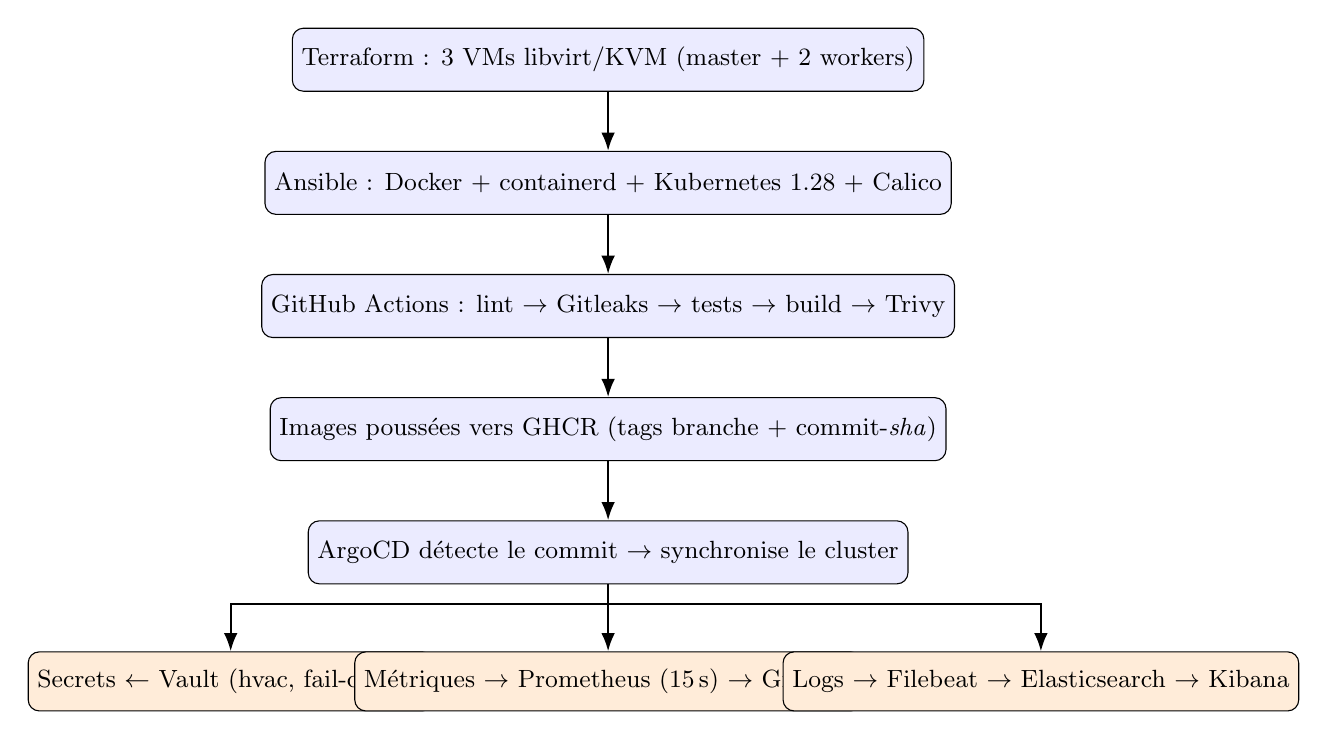
\begin{tikzpicture}[
  node distance=0.75cm and 0.9cm,
  box/.style={draw, rounded corners, fill=blue!8, minimum width=5.6cm, minimum height=0.8cm, align=center, font=\small},
  side/.style={draw, rounded corners, fill=orange!15, minimum width=3.9cm, minimum height=0.75cm, align=center, font=\small},
  arr/.style={-{Latex}, thick}
]
  \node[box] (tf) {Terraform : 3 VMs libvirt/KVM (master + 2 workers)};
  \node[box, below=of tf] (an) {Ansible : Docker + containerd + Kubernetes 1.28 + Calico};
  \node[box, below=of an] (ci) {GitHub Actions : lint $\rightarrow$ Gitleaks $\rightarrow$ tests $\rightarrow$ build $\rightarrow$ Trivy};
  \node[box, below=of ci] (ghcr) {Images poussées vers GHCR (tags branche + commit-\textit{sha})};
  \node[box, below=of ghcr] (argo) {ArgoCD détecte le commit $\rightarrow$ synchronise le cluster};
  \node[side, below left=0.85cm and -1.6cm of argo] (vault) {Secrets $\leftarrow$ Vault (hvac, fail-closed)};
  \node[side, below=0.85cm of argo] (prom) {Métriques $\rightarrow$ Prometheus (15\,s) $\rightarrow$ Grafana};
  \node[side, below right=0.85cm and -1.6cm of argo] (elk) {Logs $\rightarrow$ Filebeat $\rightarrow$ Elasticsearch $\rightarrow$ Kibana};

  \draw[arr] (tf) -- (an);
  \draw[arr] (an) -- (ci);
  \draw[arr] (ci) -- (ghcr);
  \draw[arr] (ghcr) -- (argo);
  \draw[arr] (argo.south) -- ++(0,-0.25) -| (vault.north);
  \draw[arr] (argo.south) -- (prom.north);
  \draw[arr] (argo.south) -- ++(0,-0.25) -| (elk.north);
\end{tikzpicture}%
}
\end{center}

\clearpage

% ============================================================
\section{Infrastructure : libvirt/KVM et cloud-init}
% ============================================================

\subsection{Libvirt/KVM --- hyperviseur de l'homelab}
La plateforme repose sur une virtualisation locale via \texttt{qemu:///system}. Terraform crée un réseau dédié \texttt{devops-platform-net} (domaine \texttt{devops.local}), isolé avec NAT, DHCP alloué de \texttt{192.168.56.100} à \texttt{192.168.56.200} et relais DNS vers \texttt{1.1.1.1}/\texttt{8.8.8.8}. Le sous-réseau fixé est \texttt{192.168.56.0/24} (validations Terraform : CIDR valide et plage RFC1918 uniquement).

Topologie par défaut :
\begin{itemize}[itemsep=1pt]
  \item \textbf{master-01} : \texttt{192.168.56.10} ;
  \item \textbf{worker-01} : \texttt{192.168.56.11} ; \textbf{worker-02} : \texttt{192.168.56.12} (\texttt{worker\_count} paramétrable de 1 à 32) ;
  \item chaque nœud : machine type \textbf{q35}, 2 vCPU, 4096 Mo de RAM, disque qcow2 20 Go, disque CD-ROM cloud-init, carte réseau \texttt{virtio}.
\end{itemize}

Le choix de 4 Go par nœud est documenté dans les variables : avec 2048 Mo seulement, la pile complète (ELK + ArgoCD) fait passer le kubelet en \texttt{NodeStatusUnknown} sous pression mémoire.

\begin{whybox}
KVM/libvirt offre de \emph{vraies} VM Linux sans coût cloud ni quotas, tout en restant proche d'une production (SSH, systemd, kernel réel --- pas de conteneurs-in-conteneurs). C'est l'équilibre coût/réalisme optimal pour apprendre une chaîne complète : le même code Terraform pourrait viser AWS/GCP en changeant de provider, le reste de la chaîne étant inchangé.
\end{whybox}

\subsection{Cloud-init --- durcissement au premier démarrage}
Chaque nœud reçoit un disque \texttt{cloud-init} généré depuis un template :
\begin{itemize}[itemsep=1pt]
  \item utilisateur \texttt{devops} (sudo restreint par liste blanche : uniquement \texttt{kubeadm}, \texttt{kubelet}, redémarrage \texttt{kubelet/containerd/docker}) ;
  \item \texttt{ssh\_pwauth: false}, \texttt{disable\_root: true}, \texttt{PermitRootLogin no}, authentification par clé publique seule ;
  \item installation de \textbf{fail2ban}, mise à jour complète des paquets au boot ;
  \item extension automatique de la partition racine (\texttt{growpart} + \texttt{resizefs}) ;
  \item adresse IP statique par nœud via \texttt{network-config} (DHCP désactivé).
\end{itemize}

\begin{whybox}
Cloud-init est le standard de facto du provisionnement initial (toutes les images cloud publiques le parlent). Appliquer le durcissement \emph{au boot}, avant toute intervention Ansible, garantit qu'aucune VM ne passe un seul instant dans un état faible (root SSH ouvert, mot de passe).
\end{whybox}

% ============================================================
\section{Terraform --- Infrastructure as Code}
% ============================================================

\subsection{Rôle et implémentation}
Terraform décrit l'intégralité de l'infrastructure de façon déclarative :
\begin{itemize}[itemsep=1pt]
  \item \textbf{Version épinglée} : \texttt{required\_version = "\textasciitilde> 1.5"} (CI sur matrice \texttt{1.5.7}) --- borne supérieure assumée pour éviter les ruptures de comportement des versions 1.6+ ;
  \item \textbf{Providers} : \texttt{dmacvicar/libvirt} \texttt{\textasciitilde> 0.9} (verrouillé 0.9.8) et \texttt{hashicorp/local} \texttt{\textasciitilde> 2.5} (verrouillé 2.9.0) ;
  \item ressources : réseau libvirt, volume de base qcow2, volumes par nœud, disques cloud-init, domaines (VMs) ;
  \item garde-fou \texttt{terraform\_data.ssh\_key\_guard} : échec immédiat si aucune clé publique SSH détectée (sinon les VMs naissent inaccessibles) ;
  \item \textbf{backend local} (\texttt{terraform.tfstate}) avec, en commentaire, le contrat de production prêt à l'emploi : backend S3 + verrous DynamoDB + chiffrement, activable via \texttt{-backend-config=} ;
  \item sortie \texttt{local\_file.ansible\_inventory} : rendu du template \texttt{inventory.tpl} vers \texttt{inventory.generated.ini} (jamais commité).
\end{itemize}

\subsection{Génération de l'inventaire Ansible}
L'inventaire est un \emph{artefact généré}, jamais édité à la main : \texttt{terraform refresh} puis \texttt{apply -target local\_file.ansible\_inventory}, copie ensuite dans \texttt{ansible/inventory.ini} par \texttt{scripts/generate-inventory.sh}. Cela élimine toute divergence entre l'état réel de l'infrastructure et la configuration Ansible.

\begin{whybox}
Terraform est le standard industriel de l'IaC : \texttt{plan} prévisualise les changements, l'état détecte la dérive, l'écosystème de providers couvre tout. L'épinglage \texttt{\textasciitilde> 1.5} privilégie la reproductibilité du projet sur l'actualité --- un choix défendable quand la CI rejoue exactement la même version que les développeurs. La génération de l'inventaire par Terraform supprime une classe entière d'erreurs manuelles.
\end{whybox}

% ============================================================
\section{Ansible --- configuration automatisée}
% ============================================================

\subsection{Architecture du playbook}
Un playbook unique en cinq \emph{plays}, tous avec élévation de privilèges :

\begin{enumerate}[itemsep=1pt]
  \item \texttt{all} $\rightarrow$ rôle \textbf{docker} (tag \texttt{docker}) ;
  \item \texttt{all} $\rightarrow$ rôle \textbf{k8s\_common} (pré-requis noyau et paquets) ;
  \item \texttt{masters} $\rightarrow$ rôle \textbf{k8s\_master} (initialisation du cluster) ;
  \item \texttt{workers} $\rightarrow$ rôle \textbf{k8s\_worker}, \texttt{serial: 1} (jointure séquentielle) ;
  \item \texttt{all} $\rightarrow$ rôle \textbf{k8s\_reset}, double opt-in (tag \texttt{never} \emph{et} variable \texttt{reset\_confirmed=true}) car destructif.
\end{enumerate}

Configuration : \texttt{host\_key\_checking=False} (lab), 10 forks, pipelining SSH activé, collection \texttt{community.general==8.0.0} (module \texttt{modprobe}).

\subsection{Rôle \texttt{docker}}
Ajout du dépôt Docker officiel (clé GPG dans \texttt{/etc/apt/keyrings}), installation de \texttt{docker-ce}, \texttt{docker-ce-cli}, \texttt{containerd.io} (volontairement non épinglés : les anciens pins exacts Docker 24.0.7 / containerd 1.6.21 n'existaient plus dans le dépôt apt), ajout de l'utilisateur \texttt{devops} au groupe \texttt{docker}, puis génération de \texttt{/etc/containerd/config.toml} avec bascule cruciale \texttt{SystemdCgroup = true}.

\subsection{Rôle \texttt{k8s\_common}}
\begin{itemize}[itemsep=1pt]
  \item désactivation du swap (runtime + \texttt{/etc/fstab}) ;
  \item modules noyau \texttt{overlay} et \texttt{br\_netfilter} persistés ;
  \item sysctls réseau (\texttt{bridge-nf-call-iptables}, \texttt{ip\_forward}) appliqués ;
  \item dépôt officiel \texttt{pkgs.k8s.io} : installation \textbf{épinglée} de \texttt{kubelet=1.28.*}, \texttt{kubeadm=1.28.*}, \texttt{kubectl=1.28.*}, puis \textbf{hold dpkg} sur les trois binaires (aucune montée de version accidentelle lors d'un \texttt{apt upgrade}).
\end{itemize}

\subsection{Rôles maître et workers}
\begin{itemize}[itemsep=1pt]
  \item \texttt{kubeadm init} avec CIDR pods \texttt{192.168.0.0/16}, CIDR services \texttt{10.96.0.0/12}, socket CRI containerd ; phases addon (CoreDNS, kube-proxy) \emph{différées} après l'installation du CNI pour éviter les boucles de crash initiales ;
  \item kubeconfig copié pour \texttt{devops} (mode 0600) ; attente active de l'API server (24 essais × 5\,s) ;
  \item \textbf{Calico v3.26.1} via opérateur Tigera (\texttt{-{}-server-side}), attente de disponibilité de l'opérateur puis de tous les nœuds \texttt{Ready} : échec bloquant --- un Calico cassé signifie un cluster cassé, on aborte ;
  \item commande de jointure générée avec \texttt{no\_log: true} (le token de bootstrap ne doit jamais fuiter dans les logs), stockée en mode 0600 ;
  \item les workers rejoignent via \texttt{command:} (et non \texttt{shell:}, anti-injection), garde \texttt{creates:} pour l'idempotence, attente du statut \texttt{Ready} déléguée au master.
\end{itemize}

\begin{whybox}
Ansible est agentless (SSH seul, rien à installer ni maintenir sur les nœuds), idempotent et lisible : chaque rôle documente l'état voulu plutôt que la procédure. Les choix fins --- hold dpkg, \texttt{no\_log} sur les tokens, addons différés, échec bloquant sur Calico --- traduisent une pratique de durcissement acquise par incidents réels, pas une simple exécution de tutoriel.
\end{whybox}

% ============================================================
\section{Docker et containerd --- conteneurisation}
% ============================================================

\subsection{Docker --- builds multi-stage}
Les trois services partagent un modèle de Dockerfile identique :
\begin{itemize}[itemsep=1pt]
  \item directive \texttt{syntax=docker/dockerfile:1.6} (BuildKit) ;
  \item \textbf{deux stages} : \texttt{builder} (installation des dépendances pip depuis \texttt{shared/requirements.txt} + requirements du service, purge des wheels superflues) puis image finale qui ne copie que \texttt{site-packages}, les binaires et le code ;
  \item base \texttt{python:3.11-slim} surchargeable par \texttt{-{}-build-arg BASE\_IMAGE=\ldots@sha256:\ldots} ;
  \item \textbf{non-root} : utilisateur système \texttt{appuser}, \texttt{USER appuser} avant le CMD, \texttt{COPY -{}-chown} ;
  \item \textbf{HEALTHCHECK} natif sondant \texttt{/livez} toutes les 30\,s (timeout 3\,s, période de grâce 10\,s, 3 essais) ;
  \item labels OCI (\texttt{org.opencontainers.image.source}, \texttt{licenses=MIT}) ;
  \item \textbf{contexte de build = \texttt{app/}} (jamais le répertoire du service) : indispensable puisque \texttt{shared/} est importé comme paquet de premier niveau ; le \texttt{.dockerignore} exclut \texttt{.git}, caches, états Terraform et tout ce qui ne sert pas au runtime.
\end{itemize}

\begin{whybox}
Le multi-stage divise drastiquement la taille de l'image finale (pas de pip ni de cache dans l'image livrée) et la surface d'attaque (pas d'outils de build). L'utilisateur non-root et le HEALTHCHECK sont exigés par les standards de sécurité des registres et par les probes Kubernetes : l'image est prête pour la prod, pas seulement pour la démo.
\end{whybox}

\subsection{containerd --- runtime CRI}
containerd est installé avec le cluster et configuré en pilote cgroup \texttt{systemd} (aligné sur le kubelet 1.28). C'est le runtime effectif des Pods ; Docker ne sert ici qu'à construire les images.

\begin{whybox}
Depuis la suppression de dockershim, containerd est le runtime recommandé par kubeadm : plus léger (pas de CLI ni de daemon API exposés sur les nœuds), maintenu par la CNCF, et c'est le chemin suivi par l'industrie. La configuration \texttt{SystemdCgroup=true} est obligatoire pour que kubelet et runtime partagent le même gestionnaire de cgroups.
\end{whybox}

% ============================================================
\section{Kubernetes 1.28 --- orchestration}
% ============================================================

\subsection{kubeadm et socle cluster}
Cluster amorcé par \texttt{kubeadm} (outil officiel de cycle de vie), Kubernetes \textbf{1.28}, CNI \textbf{Calico v3.26.1} (opérateur Tigera), CIDR pods/services séparés du réseau des VMs.

\begin{whybox}
kubeadm produit un cluster «conforme aux bonnes pratiques upstream», réparable et extensible --- contrairement aux distributions clés en main qui masquent la mécanique. Calico est retenu pour sa maturité, son opérateur simple et surtout ses NetworkPolicies complètes (ingress + egress), dont la plateforme dépend fortement (voir \S\ref{sec:netpol}).
\end{whybox}

\subsection{Manifestes applicatifs (Kustomize)}
Structure \texttt{k8s/apps/} : \texttt{base/} commun + un dossier par service + overlays d'environnement.

\subsubsection{Durcissement au niveau du namespace (\texttt{devops-platform})}
\begin{itemize}[itemsep=1pt]
  \item labels Pod Security Admission \texttt{enforce/audit/warn: restricted} ;
  \item \textbf{LimitRange} : défauts 250m CPU / 256 Mi (limites) et 100m / 128 Mi (requêtes), plafond absolu 4 CPU / 2 Gi ;
  \item \textbf{ResourceQuota} : 4 CPU / 4 Gi en requests, 8 CPU / 8 Gi en limits, 20 Pods/Services/ConfigMaps/Secrets, 10 PVC.
\end{itemize}

\subsubsection{Déployments (identiques pour les 3 services)}
\begin{itemize}[itemsep=1pt]
  \item 2 réplicas, RollingUpdate \texttt{maxUnavailable=1/maxSurge=1} ;
  \item \texttt{securityContext} pod : \texttt{runAsNonRoot: true}, UID/GID/fsGroup 1000, seccomp \texttt{RuntimeDefault} ; conteneur : \texttt{allowPrivilegeEscalation: false}, \textbf{\texttt{readOnlyRootFilesystem: true}}, \texttt{capabilities.drop: [ALL]} ; volume temporaire \texttt{emptyDir} sur \texttt{/tmp} ;
  \item probes : \textbf{startupProbe} sur \texttt{/livez} (tolérance 150\,s), \textbf{readiness} sur \texttt{/readyz} (vérifie la santé Vault !), \textbf{liveness} sur \texttt{/livez} ;
  \item annotations Prometheus (\texttt{prometheus.io/scrape}, port 8000, chemin \texttt{/metrics}) ;
  \item anti-affinité de pods + \texttt{topologySpreadConstraints} (maxSkew 1) : les réplicas se dispersent entre les nœuds même à petite échelle.
\end{itemize}

\subsubsection{Autoscaling et résilience}
\begin{itemize}[itemsep=1pt]
  \item \textbf{HPA} autoscaling/v2 : min 2 / max 5 réplicas, cibles 70\,\% CPU et 80\,\% mémoire ; comportement asymétrique --- montée rapide (doublement possible toutes les 30\,s, stabilisation 30\,s), descente prudente (stabilisation 300\,s, $-$25\,\% par minute) pour éviter le \emph{flapping} ;
  \item \textbf{PDB} \texttt{minAvailable: 1} (2 en prod) : les drainings et mises à jour de nœuds ne peuvent pas interrompre tous les réplicas d'un coup.
\end{itemize}

\subsection{Réseau interne : NetworkPolicies}\label{sec:netpol}
Six politiques appliquent un modèle \emph{default-deny} puis liste blanche explicite :
\begin{enumerate}[itemsep=1pt]
  \item \texttt{default-deny} : zéro ingress/egress par défaut ;
  \item egress vers Vault (namespace \texttt{vault}, TCP 8200) uniquement ;
  \item egress DNS vers \texttt{kube-system} (TCP/UDP 53) ;
  \item egresse réservée PostgreSQL futur (TCP 5432) ;
  \item ingress autorisé depuis le namespace \texttt{monitoring} (scrape métriques TCP 8000) ;
  \item ingress intra-namespace (communication inter-services).
\end{enumerate}

\begin{whybox}
Kubernetes est devenu l'API d'orchestration universelle : autoscaling, auto-réparation, rolling updates, secrets, RBAC et politiques réseau dans un seul modèle déclaratif. Les choix ci-dessus --- PSA restricted, quotas, read-only rootfs, default-deny réseau --- appliquent le principe du moindre privilège à chaque couche ; c'est exactement ce que vérifient les politiques conftest/Kyverno de la CI (\S\ref{sec:policies}).
\end{whybox}

\subsection{Overlays Kustomize}
\begin{itemize}[itemsep=1pt]
  \item \texttt{overlays/dev} : réplicas ramenés à 1 ;
  \item \texttt{overlays/staging} : namespace \texttt{staging} ;
  \item \texttt{overlays/prod} : namespace \texttt{production}, \textbf{3 réplicas}, PDB \texttt{minAvailable: 2}, tags d'images remplacés par des digests \texttt{sha256:} par la CD.
\end{itemize}

\begin{whybox}
Kustomize patche du YAML existant sans langage de template : le \texttt{base} reste lisible, chaque environnement ne déclare que ses \emph{écarts}. Natif dans \texttt{kubectl}, il s'intègre directement à ArgoCD. Helm est réservé ici aux stacks tierces (supervision), là où le paramétrage justifie réellement un moteur de templates.
\end{whybox}

\clearpage

% ============================================================
\section{Microservices FastAPI et bibliothèque partagée}
% ============================================================

\subsection{FastAPI + Uvicorn --- le socle applicatif}
Trois services (\emph{Users}, \emph{Products}, \emph{Orders}), structure volontairement identique (\texttt{main.py}, \texttt{requirements.txt}, \texttt{Dockerfile}) :
\begin{itemize}[itemsep=1pt]
  \item \textbf{FastAPI 0.139.0} servi par \textbf{Uvicorn} (\texttt{uvicorn[standard]>=0.24.0}, ASGI) sur le port 8000 ;
  \item endpoints communs : \texttt{/} (carte d'identité du service + état Vault), \texttt{/livez}, \texttt{/readyz} (503 si Vault injoignable), \texttt{/metrics} ; endpoints métier : \texttt{/users}, \texttt{/products}, \texttt{/orders} ;
  \item données de démonstration en dur (la couche métier n'est pas le sujet) ; le \texttt{DATABASE\_URL} récupéré de Vault (repli dev : sqlite en mémoire) prépare la persistance future.
\end{itemize}

\begin{whybox}
FastAPI combine validation Pydantic, documentation OpenAPI automatique, typage moderne et performances ASGI --- le meilleur rapport expressivité/légèreté pour des microservices de démonstration. Uvicorn est le serveur ASGI de référence ; \texttt{uvicorn[standard]} ajoute uvloop/httptools sans configuration.
\end{whybox}

\subsection{Bibliothèque \texttt{shared/} --- le contrat transverse}
Paquet Python installé dans chaque image (\texttt{pip install ./shared}), importé comme paquet racine :

\begin{itemize}[itemsep=2pt]
  \item \texttt{vault\_client.py} --- client \textbf{hvac 2.1.0}. Résolution du token : fichier de l'Agent Injector \texttt{/vault/secrets/token}, sinon \texttt{VAULT\_TOKEN}, sinon \texttt{VAULT\_DEV\_ROOT\_TOKEN\_ID}. Lecture KV-v2 \texttt{secret/data/devops-platform/<SERVICE\_NAME>} mise en cache processus (\texttt{lru\_cache}). Ordre \texttt{get\_secret()} : Vault $\rightarrow$ variable d'environnement $\rightarrow$ valeur par défaut $\rightarrow$ exception \texttt{SecretUnavailable}. En production, un secret introuvable fait \textbf{échouer le démarrage} (fail-closed) : jamais de JWT signé avec une clé dev prévisible. \texttt{vault\_health()} alimente \texttt{/readyz} sans jamais lever d'exception ;
  \item \texttt{log\_config.py} --- logging stdlib + \textbf{python-json-logger 2.0.7} : JSON sur stdout par défaut (\texttt{LOG\_FORMAT=json}, champs renommés \texttt{timestamp}/\texttt{level}), format humain en dev (\texttt{plain}) ;
  \item \texttt{config.py} --- dataclass \texttt{AppConfig} lisant \texttt{ENVIRONMENT}, \texttt{LOG\_FORMAT}, \texttt{VAULT\_ADDR}, \texttt{SERVICE\_NAME}.
\end{itemize}

\begin{whybox}
Centraliser secrets/logging/config dans un paquet partagé garantit que les trois services se comportent pareil (même politique fail-closed, même format de logs) et qu'un correctif se propage en un seul point. hvac est le client Vault Python de référence ; python-json-logger suffit largement face à structlog pour produire des logs parsables par ELK avec une dépendance minimale.
\end{whybox}

\subsection{Instrumentation Prometheus --- \texttt{prometheus-fastapi-instrumentator}}
Chaque service expose \texttt{/metrics} via Instrumentator 6.1.0 : histogramme HTTP par défaut (\texttt{http\_request\_duration\_seconds\_bucket}, labels \texttt{handler/method/status}), codes regroupés par classe, handlers exclus \texttt{/livez}, \texttt{/readyz}, \texttt{/metrics} pour ne pas polluer les mesures.

\begin{whybox}
Une ligne donne les métriques RED (Rate/Errors/Duration) normalisées, directement exploitables par les règles SLO (quantile p95, taux 5xx) --- là où un câblage manuel de prometheus-client aurait dupliqué du middleware fragile dans les trois services.
\end{whybox}

% ============================================================
\section{HashiCorp Vault --- gestion des secrets}
% ============================================================

\subsection{Rôle et implémentation}
Vault \textbf{1.15.2} tourne en namespace dédié \texttt{vault} (PSA baseline pour tolérer \texttt{IPC\_LOCK}). Un \textbf{Job d'amorçage} configure au premier lancement :
\begin{itemize}[itemsep=1pt]
  \item moteur KV-v2 monté sur \texttt{secret/} ;
  \item \textbf{authentification Kubernetes} (\texttt{kubernetes\_host} + CA du ServiceAccount) ;
  \item une politique par service (\texttt{vault-policy.hcl}) : lecture stricte de \texttt{secret/data/devops-platform/<svc>} (+ list sur les métadonnées), \emph{sans} capacité delete ;
  \item un rôle d'auth par service liant le ServiceAccount correspondant, TTL de token 1 h ;
  \item les entrées KV attendues : \texttt{users} (DATABASE\_URL, JWT\_SECRET\_KEY), \texttt{products} (DATABASE\_URL, API\_KEY), \texttt{orders} (DATABASE\_URL, PAYMENT\_GATEWAY\_KEY).
\end{itemize}

Le token root n'est jamais commité : le Secret \texttt{vault-root-token} est créé/roté hors bande par \texttt{bootstrap-vault-secret.sh} (génération aléatoire 64 hex, passage par stdin --- jamais en argv ni sur disque). Les Pods reçoivent \texttt{VAULT\_TOKEN} via ce Secret (référence \texttt{optional:false} : le pod ne démarre pas sans) et \texttt{VAULT\_ADDR=http://vault-service.vault.svc.cluster.local:8200}. L'Agent Injector est déjà configuré côté serveur pour la migration future (annotation par pod, fichier token).

\begin{whybox}
Vault résout le vrai problème des secrets : distribution dynamique, auditabilité, révocation, TTL courts --- là où les Secrets Kubernetes seuls sont du base64 non chiffré. L'auth Kubernetes permet à terme de supprimer tout token statique (les pods s'authentifient par leur identité de ServiceAccount). Le mode dev actuel (in-memory, auto-unseal) est assumé pour le lab ; le chemin de production (raft storage, TLS, unseal Shamir, injection par agent) est documenté dans \texttt{k8s/vault/README.md}. Le fail-closed applicatif transforme «Vault indisponible» en incident visible dès le readiness probe plutôt qu'en fuite silencieuse de secrets par défaut.
\end{whybox}

% ============================================================
\section{CI/CD : GitHub Actions et GHCR}
% ============================================================

\subsection{Déclenchements et gouvernance}
Workflow unique \texttt{.github/workflows/ci-cd.yml} :
\begin{itemize}[itemsep=1pt]
  \item \textbf{push} sur \texttt{main}, \texttt{develop}, \texttt{clean-main}, \texttt{secondary}, filtré par chemins (\texttt{app/**}, \texttt{k8s/**}, \texttt{terraform/**}, \texttt{ansible/**}, \texttt{scripts/**}, workflow, \texttt{.gitleaks.toml}) : un changement de docs seul ne déclenche rien ;
  \item \textbf{pull\_request} vers \texttt{main}/\texttt{develop}/\texttt{secondary} ; \textbf{workflow\_dispatch} manuel ; \textbf{schedule} nocturne \texttt{0 3 * * *} (détection de drift : nouvelles CVE publiées sur des dépendances déjà présentes) ;
  \item permissions globales minimales (\texttt{contents: read}), escalades par job au besoin ; concurrence \texttt{cancel-in-progress} (pas d'exécutions empilées).
\end{itemize}

\subsection{Chaîne de jobs}
\begin{lstlisting}
lint -> gitleaks -> test -> build -> trivy-scan -> deploy(manuel)
 |-> terraform-validate (parallele)
 |-> load-test (schedule uniquement)
\end{lstlisting}

\begin{description}[itemsep=2pt,leftmargin=1.4em]
  \item[lint] \texttt{ruff==0.1.9} sur \texttt{shared/} et les 3 services ; \texttt{yamllint==1.33.0} sur \texttt{k8s/} ; \texttt{terraform fmt -check -recursive} (Terraform 1.5.7) ; \textbf{kubeconform 0.6.4} valide tous les manifests contre les schémas Kubernetes 1.28.0 (hors Helm values/Chart/crds) ; \textbf{conftest} évalue les politiques Rego en mode audit.
  \item[gitleaks] scan \emph{bloquant} de l'historique complet (\texttt{fetch-depth: 0}) via \texttt{gitleaks-action@v2}, commentaires PR activés.
  \item[test] \texttt{pip-audit -{}-strict} sur chacun des 4 \texttt{requirements.txt} (toute CVE connue casse le job) ; tests pytest sous \texttt{ENVIRONMENT=dev} ; import réel de chaque \texttt{main.py} ; \textbf{builds Docker de fumée} des trois images.
  \item[build] matrice des 3 services, Buildx + cache GHA, \texttt{metadata-action} : tags \emph{branche}, \emph{commit-<sha>}, \emph{latest} uniquement sur branche par défaut, \emph{semver} ; attestations \textbf{provenance + SBOM} attachées à la poussée vers \textbf{GHCR}.
  \item[trivy-scan] matrice ×3 : rapport SARIF publié dans l'onglet Security de GitHub ; \textbf{gate bloquant} \texttt{-{}-severity CRITICAL,HIGH -{}-exit-code 1 -{}-ignore-unfixed} (types os,library) ; export SBOM SPDX en artefact (30 jours).
  \item[terraform-validate] matrice 1.5.7 : \texttt{init -backend=false} + \texttt{validate}.
  \item[deploy] \textbf{manuel uniquement}, environnement GitHub \texttt{production} : épingle les digests d'images via \texttt{kustomize edit set image}, préflight \texttt{kustomize build | kubeconform}, application \texttt{-{}-server-side} (Vault puis rendu complet), attente des rollouts (120\,s), smoke-test des \texttt{/metrics} par pod curl éphémère (\texttt{curlimages/curl:8.8.0}).
  \item[load-test] job nocturne \texttt{k6-action@v0.3.1} sur \texttt{tests/k6/load-test.js} --- fichier \textbf{pas encore écrit} : le job échoue à chaque run planifié (lacune connue et assumée).
\end{description}

\begin{whybox}
GitHub Actions vit là où vit le code : zéro infrastructure CI à maintenir, matrice native, OIDC prêt pour les backends cloud, marketplace riche. GHCR colle au dépôt (permissions héritées, packages liés aux commits). Les tags immuables (branche + sha) et l'absence de \texttt{:latest} mutable hors branche par défaut rendent chaque déploiement retraçable jusqu'au commit exact --- condition sine qua non d'un rollback fiable.
\end{whybox}

\clearpage

% ============================================================
\section{DevSecOps : sécurité intégrée au pipeline}
% ============================================================

\subsection{Gitleaks --- secrets dans le code}
Scan local (pre-commit, v8.18.0) \emph{et} CI bloquante sur tout l'historique. Configuration \texttt{.gitleaks.toml} : règles par défaut étendues, liste blanche resserrée (état Terraform exclu par défense en profondeur alors qu'il est déjà gitignored, placeholders documentés uniquement).

\begin{whybox}
La fuite de secret la plus fréquente reste le commit accidentel. Double enforcement (avant le push + sur toute l'historique en CI) attrape les deux fenêtres. Le resserrement délibéré de l'allowlist (fini les \texttt{.*\.md} exclus) montre la bonne posture : réduire les exceptions, pas les accumuler.
\end{whybox}

\subsection{Trivy --- vulnérabilités des images}
Scanner unifié CNCF : CVE OS + bibliothèques, seuil bloquant CRITICAL/HIGH sur vulnérabilités corrigeables (\texttt{ignore-unfixed}), sorties SARIF (Security tab) et SBOM SPDX conservés.

\begin{whybox}
Trivy couvre en un outil ce qui demanderait plusieurs scanners, s'intègre nativement à GitHub (SARIF) et à la supply chain (SBOM). Bloquer uniquement sur les CVE \emph{corrigeables} évite les pipelines morts-nés sur des faux positifs non réparables --- un arbitrage pragmatique documenté dans les flags mêmes du job.
\end{whybox}

\subsection{pip-audit --- dépendances Python}
Auditeur officiel PyPA, exécuté en \texttt{-{}-strict} sur les quatre fichiers de requirements : une seule dépendance épinglée avec CVE connue suffit à casser le job test.

\begin{whybox}
La chaîne d'approvisionnement Python (requirements.txt) est la surface d'attaque la plus directe du code applicatif. pip-audit interroge la base officielle des advisories ; le mode strict garantit qu'une erreur d'audit ne passe jamais inaperçue en succès silencieux.
\end{whybox}

\subsection{pre-commit --- qualité avant le push}
Onze hooks sur cinq dépôts : \texttt{check-yaml} (multi-documents autorisés pour Helm), \texttt{end-of-file-fixer}, \texttt{trailing-whitespace}, \texttt{check-merge-conflict}, \texttt{check-case-conflict}, \texttt{detect-private-key}, \texttt{ruff} (v0.1.9, fichiers \texttt{app/}+\texttt{tests/}), \texttt{yamllint} (v1.33.0), \texttt{gitleaks} (v8.18.0), \texttt{terraform\_fmt} et \texttt{terraform\_validate} (v1.92.0, \texttt{-{}-backend=false}).

\begin{whybox}
pre-commit déplace les contrôles \emph{avant} le push : le développeur corrige en secondes au lieu d'attendre un tour complet de CI. Les mêmes outils que la CI (ruff, yamllint, gitleaks, terraform) garantissent l'absence de divergence entre local et pipeline.
\end{whybox}

\subsection{Ruff, yamllint, kubeconform, conftest}\label{sec:policies}
\begin{itemize}[itemsep=2pt]
  \item \textbf{Ruff} : linter Python unique remplaçant flake8/isort/pyflakes, écrit en Rust --- assez rapide pour être exécuté à chaque sauvegarde comme en CI avec la même règle ;
  \item \textbf{yamllint} : hygiène YAML (indentation, espaces en fin de ligne) sur \texttt{k8s/} et \texttt{.github/} ;
  \item \textbf{kubeconform} : validation hors ligne contre les schémas officiels Kubernetes 1.28 (rapide, pas de cluster requis), avec exclusion propre des artefacts Helm ;
  \item \textbf{conftest/Rego} (\texttt{k8s/policies/conftest/} \texttt{security.rego}) : trois refus --- \texttt{readOnlyRootFilesystem} absent, capabilities autres que \texttt{ALL} non droppées, \texttt{runAsNonRoot} manquant. Exécuté en \emph{mode audit} (non bloquant) : la police observe avant de sanctionner ;
  \item \textbf{Kyverno} (\texttt{disallow-latest-images.yaml}) : deux ClusterPolicies en \texttt{validationFailure\allowbreak Action:\allowbreak Audit} --- images épinglées par digest, contexte de sécurité restreint. Kyverno parle «Kubernetes natif» (pas de nouveau langage) et permet une montée en charge progressive audit$\rightarrow$enforce.
\end{itemize}

\begin{whybox}
Policy-as-code transforme les bonnes pratiques de sécurité en vérifications exécutables. Le duo conftest (CI, avant déploiement) + Kyverno (cluster, au moment de l'admission) couvre les deux instants où une mauvaise config peut entrer. Commencer en audit est la bonne trajectoire industrielle : mesurer le bruit avant de bloquer.
\end{whybox}

% ============================================================
\section{ArgoCD --- GitOps}
% ============================================================

\subsection{Installation et projet}
ArgoCD \textbf{v2.7.16} installé via kustomize sur le remote base officiel \texttt{core-install} (image épinglée \texttt{quay.io/argoproj/argocd:v2.7.16}). Un \textbf{AppProject} \texttt{devops-platform} borne les droits : dépôts sources autorisés, destinations limitées aux namespaces de la plateforme, whitelist de ressources par niveau (Namespace/Service/ConfigMap au niveau cluster).

\subsection{Douze Applications, une seule source de vérité}
Chaque composant est une Application ArgoCD pointant vers son chemin Git : \texttt{argocd-install}, \texttt{observability-base}, \texttt{prometheus}, \texttt{alertmanager}, \texttt{elk}, \texttt{slo-rules}, \texttt{grafana}, \texttt{grafana-dashboards}, puis \texttt{base}, \texttt{users}, \texttt{products}, \texttt{orders}.

Politique commune : \textbf{automated + prune + selfHeal}, \texttt{CreateNamespace}, \texttt{ServerSideApply}, \texttt{PruneLast} (les suppressions passent en dernier), propagation \texttt{foreground}, retry exponentiel (5 tentatives, facteur 2). L'ordre de démarrage est garanti par des \textbf{sync waves} : $-100$ (installation d'ArgoCD elle-même) $\rightarrow$ 5 (socle monitoring) $\rightarrow$ 15 (Prometheus) $\rightarrow$ 20 (AlertManager, ELK, règles SLO) $\rightarrow$ 25 (Grafana).

\begin{whybox}
Le GitOps inverse le sens du déploiement : le cluster \emph{tire} l'état depuis Git au lieu de le recevoir d'une CI qui pousse. Conséquences concrètes : toute dérive (kubectl edit manuel) est corrigée par \texttt{selfHeal}, tout rollback est un \texttt{git revert}, l'état complet du système est auditable dans l'historique Git. Les sync waves résoluent élégamment le bootstrapping ordonné (Prometheus doit exister avant que Grafana cherche sa datasource). ServerSideApply évite les collisions de champs entre gestionnaires.
\end{whybox}

\clearpage

% ============================================================
\section{Observabilité : Prometheus, Grafana, ELK}
% ============================================================

\subsection{Prometheus (Operator) --- collecte de métriques}
Deux voies fournies : chart Helm parapluie (\texttt{prometheus-community/prometheus} 25.8.0) ou --- voie active pilotée par ArgoCD --- \textbf{Prometheus Operator 0.74.0} + CRDs, instance Prometheus \textbf{v2.51.0} : rétention 15 j (PVC local-path 10 Gi, cap 8 GiB), \textbf{scrapeInterval 15\,s} aligné sur les ServiceMonitors (scrapeTimeout 10\,s), alertes routées vers AlertManager.

Découverte automatique par \textbf{ServiceMonitor} : chaque service publie le sien (namespace \texttt{devops-platform}, port \texttt{http}, chemin \texttt{/metrics}, 15\,s). Compléments : \textbf{kube-state-metrics v2.10.1} (état des objets : réplicas, HPA, OOMKills\ldots) et scrape explicite des kubelets (\texttt{/metrics/cadvisor}, IP fixes \texttt{192.168.56.10--12}, TLS avec skip-verify assumé pour le lab).

\begin{whybox}
L'Operator transforme la configuration de Prometheus en ressources Kubernetes déclaratives : ajouter un service supervisé revient à poser un ServiceMonitor --- exactement ce que le modèle GitOps sait synchroniser. kube-state-metrics fournit les métriques indispensables aux alertes plateforme (HPA bloqué, évictions OOM) que Prometheus ne voit pas seul.
\end{whybox}

\subsection{AlertManager --- routage des alertes}
AlertManager \textbf{v0.27.0} : groupement par \texttt{alertname/service}, \texttt{groupWait 30s}, \texttt{groupInterval 5m}, \texttt{repeatInterval 4h} ; receiver webhook vide (TODO Slack/PagerDuty documenté).

Règles SLO (\texttt{rules.yaml}) --- le cœur opérationnel :

\begin{table}[h!]
\centering\small
\begin{tabular}{@{}llll@{}}
\toprule
\textbf{Alerte} & \textbf{Condition} & \textbf{for} & \textbf{Gravité} \\
\midrule
SLOAvailabilityBreach & dispo.\ 30j $<$ 99{,}9\,\% & 10 min & critical \\
SLOLatencyP95Breach & p95 $>$ 200 ms & 5 min & warning \\
SLO5xxErrorRateBreach & taux 5xx $>$ 1\,\% & 2 min & critical \\
ContainerMemoryRatioHigh & RAM $>$ 80\,\% de la limite & 2 min & warning \\
PodEvictionOngoing & OOMKill détecté & 1 min & critical \\
HPAPinnedAtMaxReplicas & HPA collé au max 15 min & 15 min & warning \\
\bottomrule
\end{tabular}
\caption{Règles d'alerte SLO et plateforme}
\end{table}

La disponibilité 30 jours s'appuie sur une \textbf{recording rule} (\texttt{service:availability\_30d:ratio} par \texttt{avg\_over\_time(up[30d])}) : la requête coûteuse est pré-calculée toutes les 5 minutes.

\begin{whybox}
Des SLO chiffrés (disponibilité, latence p95, erreurs) transforment la supervision subjective en contrat mesurable --- les mêmes chiffres figurent dans ce rapport (\S\ref{sec:slo-table}) et dans les règles. Les alertes «incident» (OOMKill, HPA saturé) correspondent aux scénarios réels rencontrés pendant le projet : on alerte sur ce qui est déjà arrivé.
\end{whybox}

\subsection{Grafana --- visualisation}
Grafana \textbf{11.1.0} : deux datasources provisionnées en ConfigMap (Prometheus, intervalle 15\,s ; Elasticsearch 8.14.0 sur l'index \texttt{devops-platform-*}), credentials injectés hors bande (Secret + variables \texttt{\_FILE}), inscription anonyme désactivée. Les dashboards sont du \textbf{code} : quatre ConfigMaps labellisés (\texttt{grafana\_dashboard="1"}) chargés par le sidecar \texttt{kiwigrid/k8s-sidecar:1.27.6} --- \emph{Infrastructure Overview}, \emph{Application Performance} (RPS, p95/p99, heatmap), \emph{Error Rate SLO} (ligne de seuil 1\,\%), \emph{Infrastructure Detail} (saturation mémoire, OOMKills, HPA).

\begin{whybox}
Dashboards-as-code = reviewables en PR, versionnés, restaurables, synchronisés par ArgoCD comme tout autre manifest. Le sidecar élimine l'export/import manuel JSON : la vérité reste dans Git.
\end{whybox}

\subsection{ELK Stack 8.14 --- logs centralisés}
\begin{itemize}[itemsep=2pt]
  \item \textbf{Elasticsearch 8.14.0} : StatefulSet mono-nœud, sécurité xpack activée (HTTP), heap JVM 512 Mo calibré pour la VM 4 Go, PVC 10 Gi local-path ;
  \item \textbf{Filebeat 8.14.0} en DaemonSet : autodiscovery des Pods par hints Kubernetes (condition \emph{part-of: devops-platform}), lecture hostPath \texttt{/var/log} + logs conteneurs, envoi \textbf{direct à Elasticsearch} (queue mémoire 4096 événements) ;
  \item \textbf{Logstash 8.14.0} déployé également (entrée Beats 5044, filtre JSON, enrichissement métadonnées, \emph{drop} des requêtes de santé \texttt{/livez//readyz}, index quotidien \texttt{devops-platform-*}, queue persistée) ;
  \item \textbf{Kibana 8.14.0} : recherche/exploration, télémétrie désactivée, épinglé sur worker-01.
\end{itemize}

Credentials Elasticsearch/Kibana créés par \texttt{bootstrap-elasticsearch-secret.sh} (fichier temporaire 0600 + trap de nettoyage, jamais en argv).

\begin{whybox}
Les métriques disent \emph{qu'il y a} un problème ; les logs disent \emph{pourquoi}. ELK reste la référence open-source complète (collecte, enrichissement, stockage plein-texte, exploration). Filebeat en DaemonSet est le pattern standard de collecte nodale ; l'autodiscovery par labels fait que tout nouveau Pod de la plateforme est loggé sans configuration. La stack est dimensionnée au plus juste (heaps JVM réduits, queues bornées) pour tenir dans l'homelab --- contrainte réelle de production apprise tôt.
\end{whybox}

\subsection{SLO --- objectifs de service}\label{sec:slo-table}
\begin{table}[h!]
\centering
\begin{tabular}{@{}ll@{}}
\toprule
\textbf{SLI} & \textbf{SLO} \\
\midrule
Disponibilité & $\geq$ 99{,}9\,\% sur 30 jours \\
Latence p95 & $<$ 200 ms \\
Taux d'erreurs 5xx & $<$ 1\,\% \\
MTTD & $<$ 2 min \\
MTTR & $<$ 30 min \\
\bottomrule
\end{tabular}
\caption{Objectifs de niveau de service implémentés dans les règles AlertManager}
\end{table}

% ============================================================
\section{Exploitation : scripts de validation}
% ============================================================

\subsection{\texttt{validate-platform.sh} --- 7 contrôles de bout en bout}
Flags : \texttt{-{}-ci} (exit 1, outil manquant = échec et non skip), \texttt{-{}-only}, \texttt{-{}-skip-incident}, \texttt{-{}-namespace}, \texttt{-{}-image-tag}. Contrôles :
\begin{enumerate}[itemsep=1pt]
  \item cluster Kubernetes opérationnel (tous les nœuds Ready) ;
  \item pods des services en Running (readyReplicas = réplicas voulus) ;
  \item aucune vulnérabilité critique (Trivy CRITICAL/HIGH, exit-code 1) ;
  \item aucun secret détecté (Gitleaks, historique complet) ;
  \item ArgoCD synchronisé (Applications Synced + Healthy) ;
  \item dashboards Grafana actifs (déploiement prêt + $\geq$3 ConfigMaps labellisés) ;
  \item logs indexés dans ELK (ES healthy, Filebeat complet, Kibana prêt).
\end{enumerate}
Bonus A \emph{Self-healing} : supprime volontairement un pod et exige sa recréation en moins de 30 s (destructif, désactivable).

\subsection{\texttt{validate-security.sh} --- 4 contrôles sécurité}
(1) Gitleaks zéro secret ; (2) Trivy par image ; (3) Vault initialisé \emph{et} déscellé (\texttt{vault status}); (4) preuve de vie du token root : lecture du Secret, rejet des placeholders, \texttt{vault token lookup} dans le pod avec affichage du TTL.

\subsection{Autres outils d'exploitation}
\texttt{smoke-test.sh} (parcours E2E : pods, endpoints via port-forward, targets Prometheus, santé Grafana) ; \texttt{stress-hpa.sh} (charge Apache Bench \texttt{-c 80 -n 4000}, vérification du scale 2$\rightarrow$5) ; \texttt{stress-panel.py} (petite UI stdlib de pilotage) ; \texttt{generate-inventory.sh} ; \texttt{bootstrap-vault-secret.sh} et \texttt{bootstrap-elasticsearch-secret.sh} (création/rotation de secrets sans exposition argv/disque/git).

\begin{whybox}
Une plateforme non vérifiable n'existe pas : ces scripts encodent la définition de «ça marche» et servent à la fois de recette locale, de garde CI (\texttt{-{}-ci}) et de démonstration en entretien. Le bonus self-healing teste le comportement --- pas la config : c'est le seul moyen de prouver que l'auto-réparation Kubernetes fonctionne réellement.
\end{whybox}

\clearpage

% ============================================================
\section{Tableau récapitulatif des technologies}
% ============================================================

{\small
\begin{longtable}{@{}p{3.1cm}p{2.0cm}p{4.6cm}p{4.6cm}@{}}
\caption{Toutes les technologies du projet : version, rôle, raison du choix}\label{tab:recap}\\
\toprule
\textbf{Outil} & \textbf{Version} & \textbf{Ce qu'il fait ici} & \textbf{Pourquoi lui} \\
\midrule
\endfirsthead
\toprule
\textbf{Outil} & \textbf{Version} & \textbf{Ce qu'il fait ici} & \textbf{Pourquoi lui} \\
\midrule
\endhead
\bottomrule
\endlastfoot
Libvirt/KVM & QEMU-KVM & 3 VMs (q35, virtio, réseau NAT dédié) & Virtualisation locale réaliste, gratuite, reproductible \\
cloud-init & Ubuntu 22.04 img & Provisionnement + durcissement au boot & Standard du first-boot, durcissement avant tout le reste \\
Terraform & $\sim$1.5 (CI 1.5.7) & IaC : réseau, volumes, VMs, inventaire & Standard IaC, plan/état/dérive, providers verrouillés \\
Provider libvirt & 0.9.8 & Piloter KVM depuis Terraform & Seul provider KVM mature de l'écosystème \\
hashicorp/local & 2.9.0 & Rendre le fichier d'inventaire & Génération d'artefacts locaux idempotente \\
Ansible & + collection 8.0.0 & Config : Docker, K8s, jointure, CNI & Agentless, idempotent, rôles lisibles \\
Docker CE & repo officiel & Construire les images (multi-stage) & Référence des builds d'images OCI \\
containerd & repo officiel & Runtime CRI des Pods & Runtime recommandé par kubeadm, léger \\
Kubernetes & 1.28 (dpkg held) & Orchestration, autoscaling, auto-réparation & API universelle de l'orchestration \\
kubeadm & 1.28 & Cycle de vie du cluster & Outil officiel, cluster conforme upstream \\
Calico & v3.26.1 (Tigera) & CNI : routes pods + NetworkPolicies & Mature, policies ingress+egress complètes \\
Kustomize & 5.4.3 (CI/deploy) & Base + overlays dev/staging/prod & Patch sans template, natif kubectl/ArgoCD \\
FastAPI & 0.139.0 & Framework HTTP des 3 services & Validation Pydantic, OpenAPI auto, async \\
Uvicorn & $>=$0.24 [standard] & Serveur ASGI (port 8000) & Serveur ASGI de référence \\
hvac & 2.1.0 & Client Vault Python & Client de référence pour KV-v2 + auth K8s \\
python-json-logger & 2.0.7 & Logs JSON stdout & Structuré pour ELK, dépendance minimale \\
prometheus-fastapi-instrumentator & 6.1.0 & Métriques RED sur /metrics & Une ligne = histogramme HTTP normalisé \\
Vault & 1.15.2 (dev mode) & Secrets dynamiques, auth Kubernetes, TTL 1h & Distribution, rotation, révocation \\
GitHub Actions & --- & Pipeline CI/CD + jobs nocturnes & CI native du dépôt, matrice, OIDC-ready \\
GHCR & ghcr.io & Registre des images & Colocalisé au dépôt, permissions héritées \\
Gitleaks & 8.18.0 (action v2) & Détection de secrets (local + CI bloquant) & Scan rapide de tout l'historique, config maison \\
Trivy & action v0.24.0 & Scan CVE bloquant + SARIF + SBOM & Scanner unifié, intégration Security tab \\
pip-audit & --- (--strict) & Audit des requirements Python & Officiel PyPA, base d'advisories officielle \\
Ruff & 0.1.9 & Linter Python & Ultra-rapide, remplace 3 outils \\
yamllint & 1.33.0 & Hygiène YAML & Standard simple, intégré pre-commit+CI \\
kubeconform & 0.6.4 & Validation schémas K8s 1.28 & Hors ligne, rapide, exclusions Helm propres \\
conftest (Rego) & --- (mode audit) & Politiques sécurité manifests & Policy-as-code avant admission \\
Kyverno & --- (Audit) & Policies cluster (digest, securityContext) & Natif Kubernetes, montée audit$\to$enforce \\
pre-commit & 11 hooks & Qualité avant push (5 dépôts) & Shift-left, mêmes règles qu'en CI \\
ArgoCD & v2.7.16 & GitOps pull, prune, selfHeal, waves & État du cluster = Git, rollback = git revert \\
Prometheus Operator & 0.74.0 & CRDs ServiceMonitor, PrometheusRule & Découverte déclarative compatible GitOps \\
Prometheus & v2.51.0 & Collecte 15 s, rétention 15 j, recording rules & Standard des métriques, langage PromQL \\
kube-state-metrics & v2.10.1 & Métriques des objets cluster & Source des alertes HPA/OOM \\
AlertManager & v0.27.0 & Groupement/routage des alertes & Routage standard de l'écosystème Prometheus \\
Grafana & 11.1.0 & Dashboards provisionnés par sidecar & Dashboards-as-code versionnés \\
kiwigrid sidecar & 1.27.6 & Chargement des dashboards ConfigMap & Provisionnement automatique sans import manuel \\
Elasticsearch & 8.14.0 & Stockage/recherche des logs & Plein-texte, référence de la stack ELK \\
Filebeat & 8.14.0 (DaemonSet) & Collecte logs nœuds/Pods & Autodiscovery K8s, pattern standard \\
Logstash & 8.14.0 & Enrichissement/filtrage (drop healthchecks) & Pipeline de transformation des events \\
Kibana & 8.14.0 & Exploration des logs & Interface de recherche standard ELK \\
Apache Bench & ab -c80 -n4000 & Génération de charge (test HPA) & Zéro dépendance, suffisant pour scaler \\
k6 & action v0.3.1 & Test de charge scripté nocturne & Scénarios JS versionnés (script à écrire) \\
jq/curl & --- & Manipulation JSON dans les scripts & Bases de tout scripting d'exploitation \\
\end{longtable}
}

% ============================================================
\section{Limites connues et axes d'amélioration}
% ============================================================

Lecture honnête du code actuel :
\begin{itemize}[itemsep=2pt]
  \item \texttt{tests/k6/load-test.js} n'existe pas : le job nocturne \texttt{load-test} échoue systématiquement --- priorité d'écriture ;
  \item le job \texttt{deploy} lit \texttt{needs.build.outputs.image} (une chaîne unique issue d'une matrice de 3 lignes : dernière ligne gagnante) --- limitation documentée inline ;
  \item \texttt{trivy-scan} résout les images par tag (\texttt{github.ref\_name}) et non par digest malgré l'intention affichée ;
  \item Vault reste en mode dev (in-memory, auto-unseal, token root partagé) : le durcissement raft/TLS/injector est planifié mais non câblé côté Pods ;
  \item l'overlay dev patche les réplicas à 1 sans retirer les HPA (min 2) : conflit latent ;
  \item l'AppProject ArgoCD conserve des destinations istio-system/flagger-system héritées de la stack canary supprimée ;
  \item Filebeat est commenté comme envoyant vers Logstash:5044 alors qu'il écrit directement dans Elasticsearch (Logstash déployé en parallèle, prêt à s'intercaler) ;
  \item corruption cosmétique d'accents dans quelques chaînes de \texttt{validate-platform.sh} (logique intacte) ;
  \item checksum du manifest Tigera non vérifié (TODO inline), \texttt{host\_key\_checking=False} assumé pour le lab.
\end{itemize}

% ============================================================
\section{Conclusion}
% ============================================================

DevOps Central Platform démontre qu'une chaîne DevOps professionnelle complète peut tenir dans un homelab : Terraform provisionne, cloud-init durcit, Ansible installe, Docker empaquette, Kubernetes orchestre, GitHub Actions vérifie et pousse, Trivy/Gitleaks/pip-audit filtrent la supply chain, Vault distribue les secrets en fail-closed, ArgoCD maintient Git comme unique source de vérité, Prometheus/Grafana/ELK rendent le tout observable et les SLO le rendent contractuel.

Chaque outil a été choisi pour une raison précise et documentée ici --- et les limites restantes sont listées tout aussi explicitement : c'est cette double honnêteté (ce qui marche, ce qui manque, pourquoi) qui fait du projet un véritable exercice d'ingénierie plutôt qu'un assemblage de tutoriels.

\end{document}
